\documentclass{article}

\usepackage{amsmath}
\usepackage{amssymb}
\usepackage[spanish]{babel}
\usepackage[margin=1.5in]{geometry}
\usepackage{graphicx}
\usepackage[utf8]{inputenc}

\renewcommand{\Bbb}{\mathbb}

\begin{document} 

\section{Práctica 1 - Cónicas en $\Bbb R^2$ y planos en $\Bbb R^3$}

\subsection{Cónicas}

Las cónicas son curvas planas (bidimensionales) que se obtienen al seccionar un cono (tridimensional) de diferentes maneras.

\subsubsection{Circunferencia}

\begin{equation}
(x-x_0)^2 + (y-y_0)^2 = r^2, \text{ siendo r el radio y } (x_0, y_0) \text{ el centro}
\end{equation}

\subsubsection{Elipse}

\begin{equation}
\frac{(x-x_0)^2}{a^2} + \frac{(y-y_0)^2}{b^2} = 1, \text{ siendo a el semieje x, b el semieje y, y } (x_0, y_0) \text{ el centro}
\end{equation}

\subsubsection{Parábolas}

Parábola vertical:

\begin{equation}
y = a (x-c)^2 + b
\end{equation}

Parábola horizontal:

\begin{equation}
x = a (y-c)^2 + b
\end{equation}

\subsubsection{Hipérbolas}

\begin{equation}
\frac{(x-x_0)^2}{a^2} - \frac{(y-y_0)^2}{b^2} = 1
\end{equation}

\begin{figure}[t]
\caption{Hipérbolas}
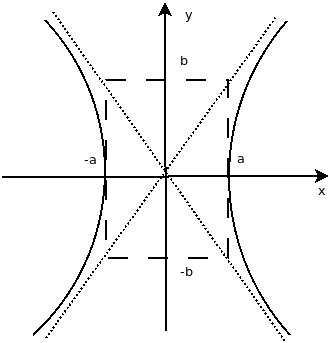
\includegraphics[scale=0.8]{img/pra_fig001_hiperbolas.png} 
\centering
\label{fig:hiperbolas}
\end{figure}

En la hipérbola de la figura ~\ref{fig:hiperbolas}, $a$ es el semilado $x$ del rectángulo, y $b$ corresponde al semilado $y$. El centro del rectángulo es el punto $(x_0, y_0)$, que en el dibujo corresponde al origen. 
Nótese además que las diagonales del rectángulo definido por $a$ y $b$ son asíntotas oblicuas de la cónica. Por otro lado, el eje que la curva no corta es el asociado al término negativo ($y$ en este ejemplo).

\subsection{Planos}

La \textbf{forma implícita} de definir un plano en $\Bbb R^3$ es:

\begin{equation}
\overline{N} \cdot (\overline{Q} - \overline{P}) = 0
\end{equation}

En este esquema, $P$ y $Q$ son dos puntos pertenecientes al plano, y $N$ es la \textbf{normal}, un vector ortogonal al plano.

Por otro lado, se tiene la \textbf{forma vectorial}:

\begin{equation}
(x,y,z) = \alpha (p_1, p_2, p_3) + \beta (q_1, q_2, q_3) + R
\end{equation}

En esta forma, $P = (p_1, p_2, p_3)$ y $Q = (q_1, q_2, q_3)$ son dos vectores, no puntos; es importante la distinción en este caso; pensar a los vectores como segmentos orientados para distinguirlos de los puntos. De ese modo, $P$ y $Q$ son vectores contenidos en el plano, en tanto $R$ es un punto contenido en el mismo. Los parámetros $\alpha$ y $\beta$ son reales, y sus combinaciones de valores cubren todo el plano definido. 

\section{Práctica 2 - Coordenadas polares - Cuádricas}

\subsection{Coordenadas polares}

En el sistema de coordenadas cartesianas en $\Bbb R^2$, se miden las proyecciones del vector posición sobre el eje $x$ y el eje $y$. En cambio, en el sistema de coordenadas polares, se miden el ángulo respecto al eje $x$ (coordenada $\phi$), y la distancia desde el origen al punto sobre la recta asociada a dicho ángulo (coordenada $\rho$).

\begin{figure}[t]
\caption{Coordenadas polares}
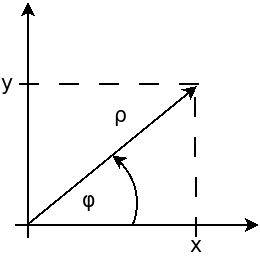
\includegraphics[scale=1.0]{img/pra_fig002_polares.png} 
\centering
\label{fig:polares}
\end{figure}

Conversión de C.C. a C.P.:

\begin{subequations}
\begin{align}
x & = \rho \cos \phi \\
y & = \rho \sin \phi
\end{align}
\end{subequations}

Conversión de C.P. a C.C.:

\begin{subequations}
\begin{align}
\rho & = \sqrt{x^2 + y^2} \\
\phi & = \arctan \left( \frac{y}{x} \right)
\end{align}
\end{subequations}

\subsection{Cuádricas}

Las cuádricas son superficies en $\Bbb R^3$ que encierran un volumen.

\subsubsection{Esfera}

\begin{equation}
(x-x_0)^2 + (y-y_0)^2 + (z-z_0)^2 = r^2
\end{equation}

\subsubsection{Elipsoide}

\begin{equation}
\frac{(x-x_0)^2}{a^2} + \frac{(y-y_0)^2}{b^2} + \frac{(z-z_0)^2}{c^2} = 1
\end{equation}

\subsubsection{Paraboloide}

\begin{equation}
\frac{(x-x_0)^2}{a^2} + \frac{(y-y_0)^2}{b^2} = z
\end{equation}

Con esta definición, el paraboloide se proyecta sobre $z$ (puede ser sobre $x$ o $y$, intercambiando las variables).

\subsubsection{Cilindro}

Circular recto, sobre el eje $z$:

\begin{equation}
(x-x_0)^2 + (y-y_0)^2 = r^2, z \in \Bbb R
\end{equation}

Elíptico recto, sobre el eje $z$:

\begin{equation}
\frac{(x-x_0)^2}{a^2} + \frac{(y-y_0)^2}{b^2} = 1, z \in \Bbb R
\end{equation}

\subsubsection{Cono}

Circular:

\begin{equation}
(x-x_0)^2 + (y-y_0)^2 = (z-z_0)^2
\end{equation}

Elíptico:

\begin{equation}
\frac{(x-x_0)^2}{a^2} + \frac{(y-y_0)^2}{b^2} = (z-z_0)^2
\end{equation}

\subsubsection{Hiperboloide (1 hoja)}

\begin{equation}
\frac{(x-x_0)^2}{a^2} + \frac{(y-y_0)^2}{b^2} - \frac{(z-z_0)^2}{c^2} = 1
\end{equation}

\begin{figure}[t]
\caption{Hiperboloide (1 hoja)}
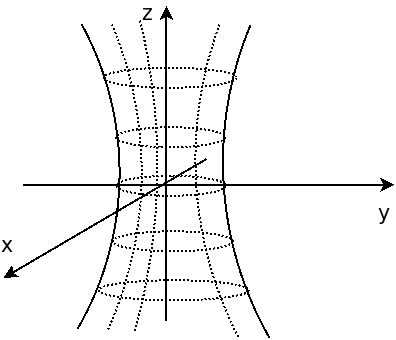
\includegraphics[scale=0.75]{img/pra_fig003_hiperboloide1.png} 
\centering
\label{fig:hiperboloide1}
\end{figure}

\subsubsection{Hiperboloide (2 hojas)}

\begin{equation}
-\frac{(x-x_0)^2}{a^2} - \frac{(y-y_0)^2}{b^2} + \frac{(z-z_0)^2}{c^2} = 1
\end{equation}

\begin{figure}[t]
\caption{Hiperboloide (2 hojas)}
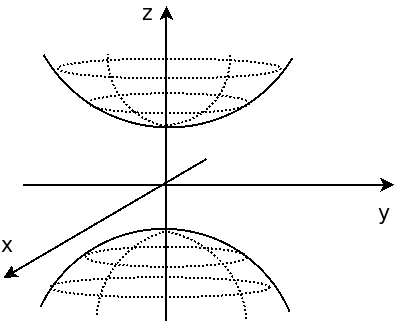
\includegraphics[scale=0.75]{img/pra_fig004_hiperboloide2.png} 
\centering
\label{fig:hiperboloide2}
\end{figure}

\subsubsection{Paraboloide hiperbólico}

\begin{equation}
-\frac{(x-x_0)^2}{a^2} + \frac{(y-y_0)^2}{b^2} = \frac{z-z_0}{c}
\end{equation}

\begin{figure}[t]
\caption{Paraboloide hiperbólico}
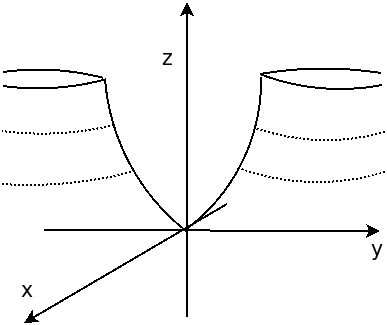
\includegraphics[scale=0.75]{img/pra_fig005_paraboloide_h.png} 
\centering
\label{fig:paraboloide_h}
\end{figure}

\end{document} 
